\section*{Results}

Due to time constraints and under-budgeting, the actual sample size for this research is smaller than initially proposed. The original proposal estimated a small sample population of three to five of the most common, accessible serial printers. However, the shipment of additional printers would have taken longer than the submission deadline. All data presented is limited to available equipment at the time of reporting, the SNBC BTP-S80 serial printer.

\subsection{Device Disassembly} \label{devicedisassembly}

% \textbf{Outline}
% $\downarrow$

% \begin{itemize}
%     \item Walkthrough of documented teardown of the serial printer
%     \item Show pictures of each stage/device layers
%     \item Label pictures indicating functionality for regions of each layer (power deliver, data, I/O...)
%     \item Provide labeled key to refer in later sections
%     \item Could manufacturer increased physical security (?)
% \end{itemize}

% \textbf{The random ipsum lorem text is to gauge how much will be written when done. This will appear several times throughout the outline.}

The SNBC BTP-S80 is a common thermal printer used for providing receipts for PoS systems and immediate reporting for industrial control systems (ICS). This model features three buttons on the front face of the printer. Starting from the top: paper roll release, auto-feeding, and power button.  

\begin{figure}[ht]
    \centering
    {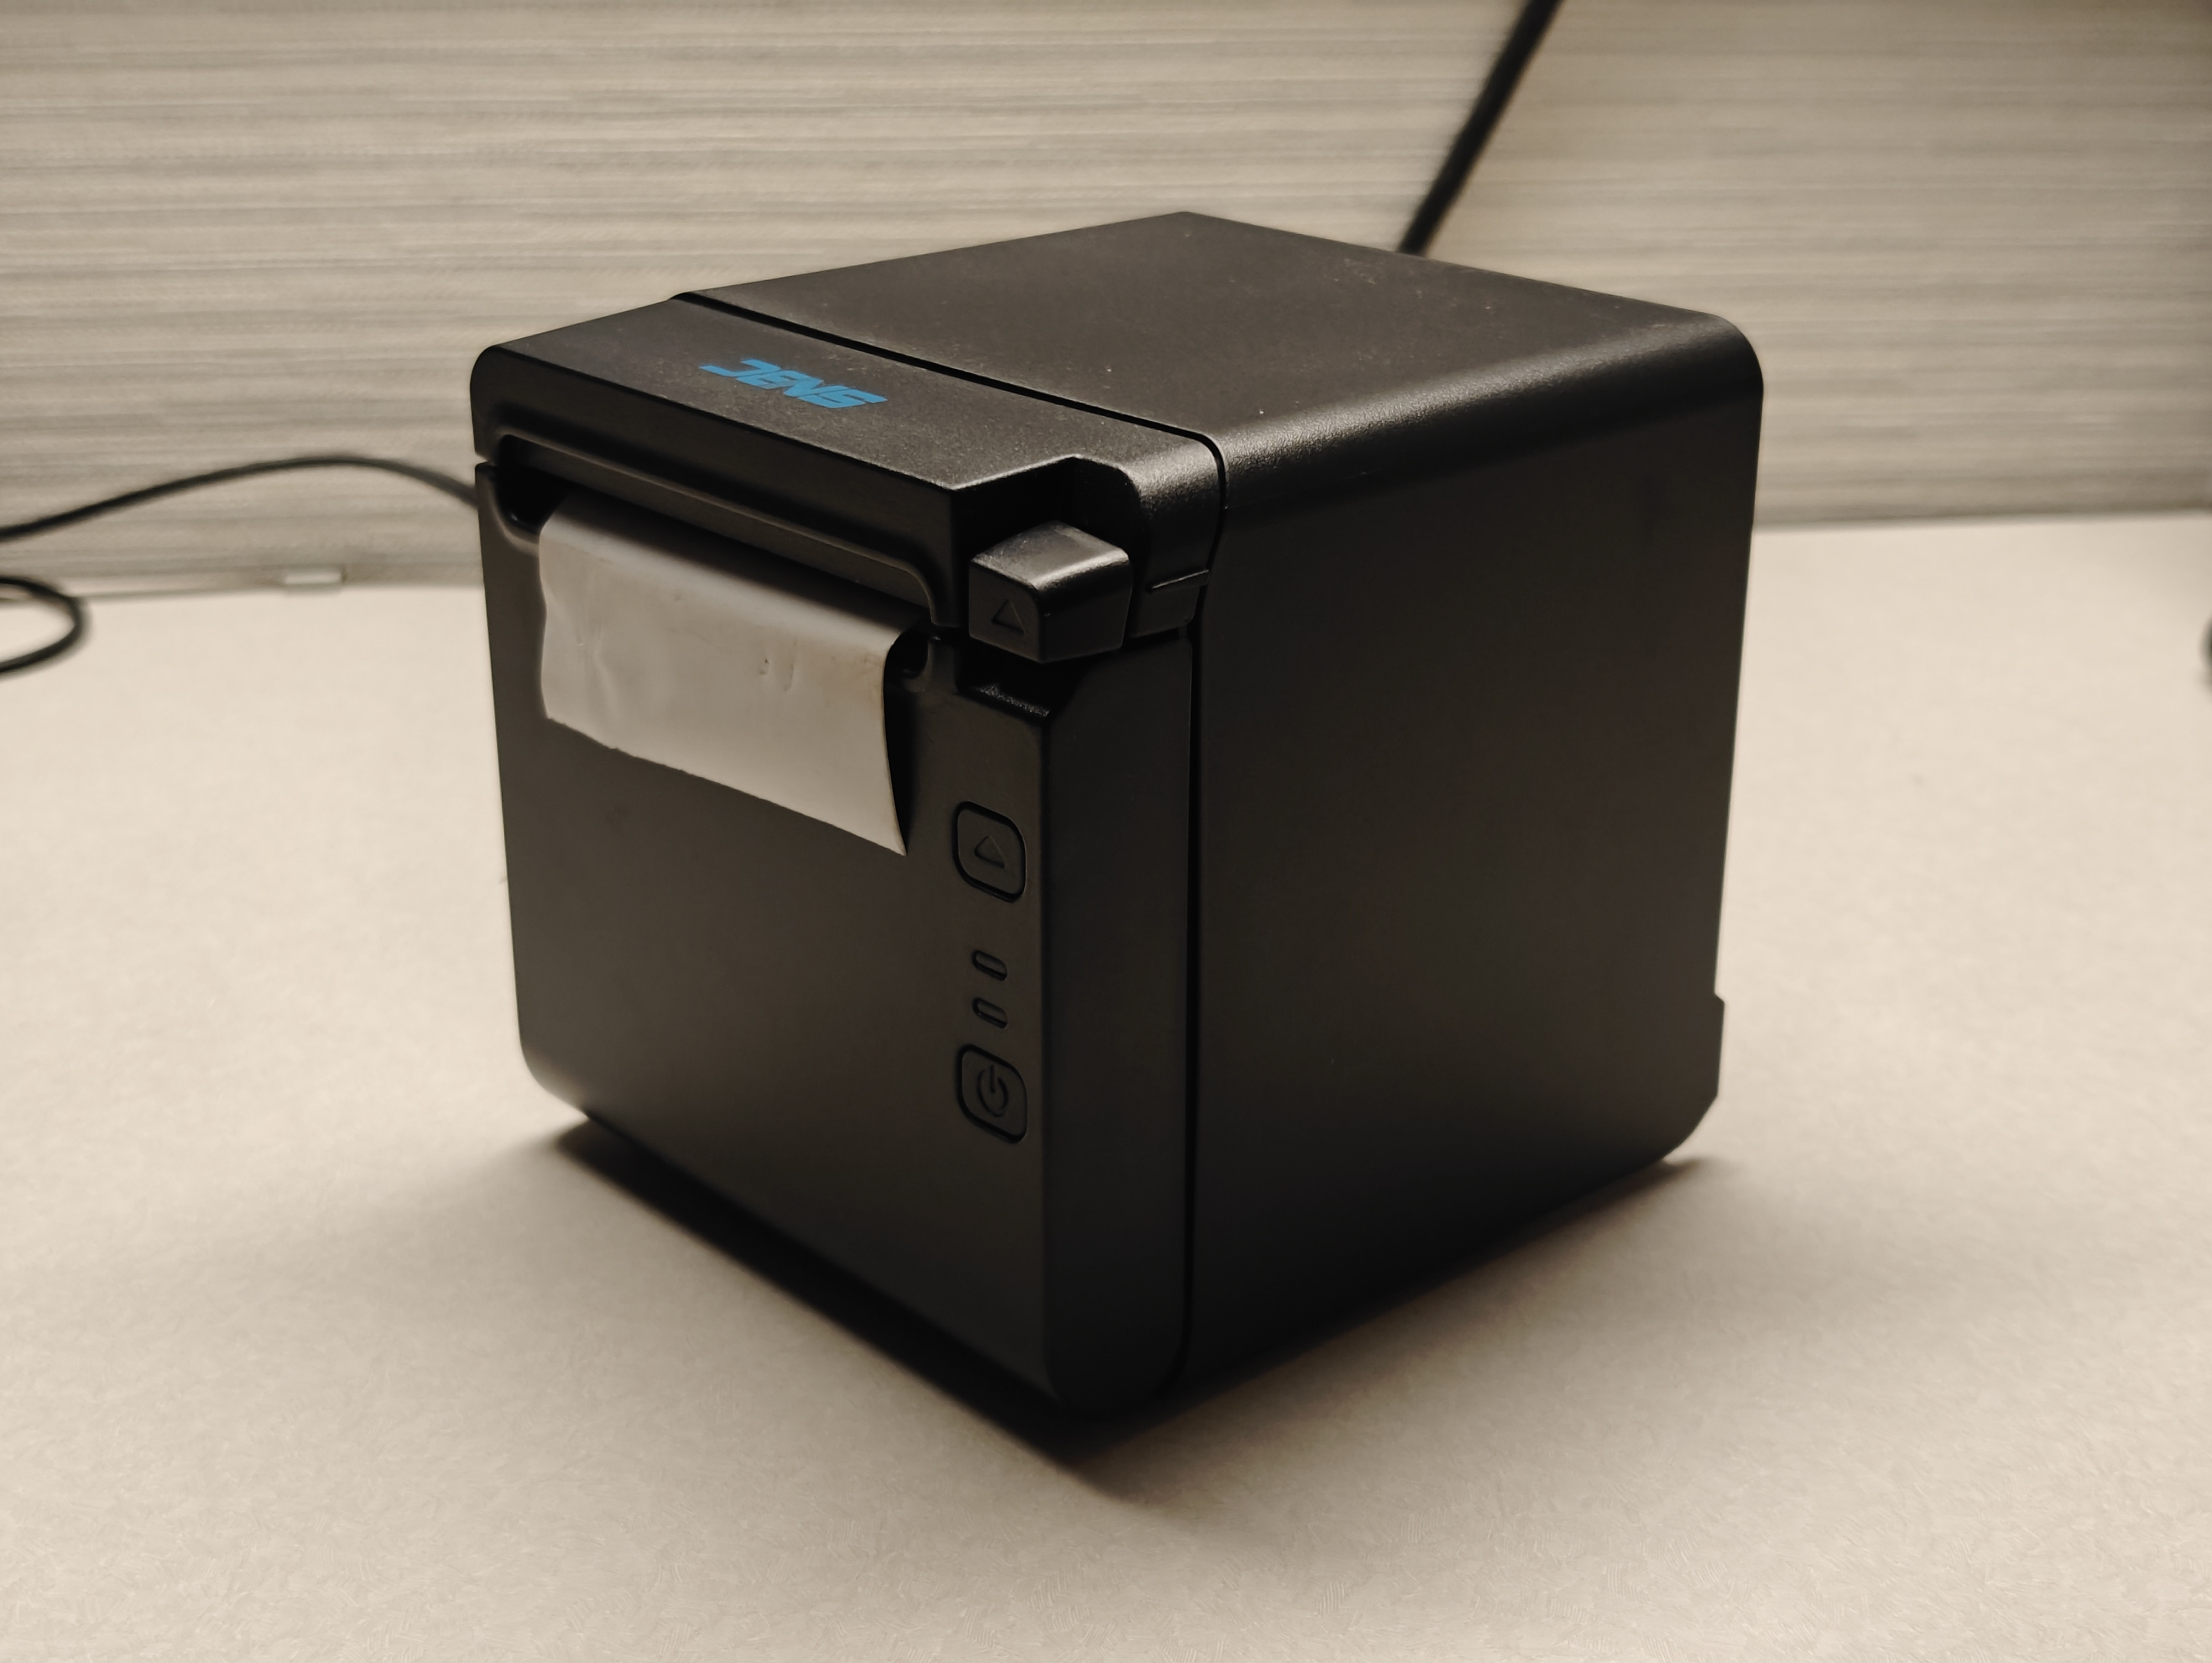
\includegraphics[width=88mm,scale=0.5]
    {Figures/Teardown/IMG20231204170511.jpg}}
    \caption{SNBC BTP-S80}
    \label{fig:snbc_btp_s80}
\end{figure}

From the rear of the device, we can see some of the available I/O. There are several ways to interface with the thermal printer. The host device can connect using an internet address via the RJ45 ethernet connector or over serial using the USB type-b and RS232. We can also see a screw on either side of the expansion card containing the RJ45 jack and RS232 connector. The manufactures website shows that this slot is interchangeable and can provide different functionality depending on the end-users needs. Some configurations are setup as shown in Figure \ref{fig:snbc_btp_s80_io}, others feature wireless adapters utilizing 2.4Ghz networking.

\begin{figure}[ht]
    \centering
    {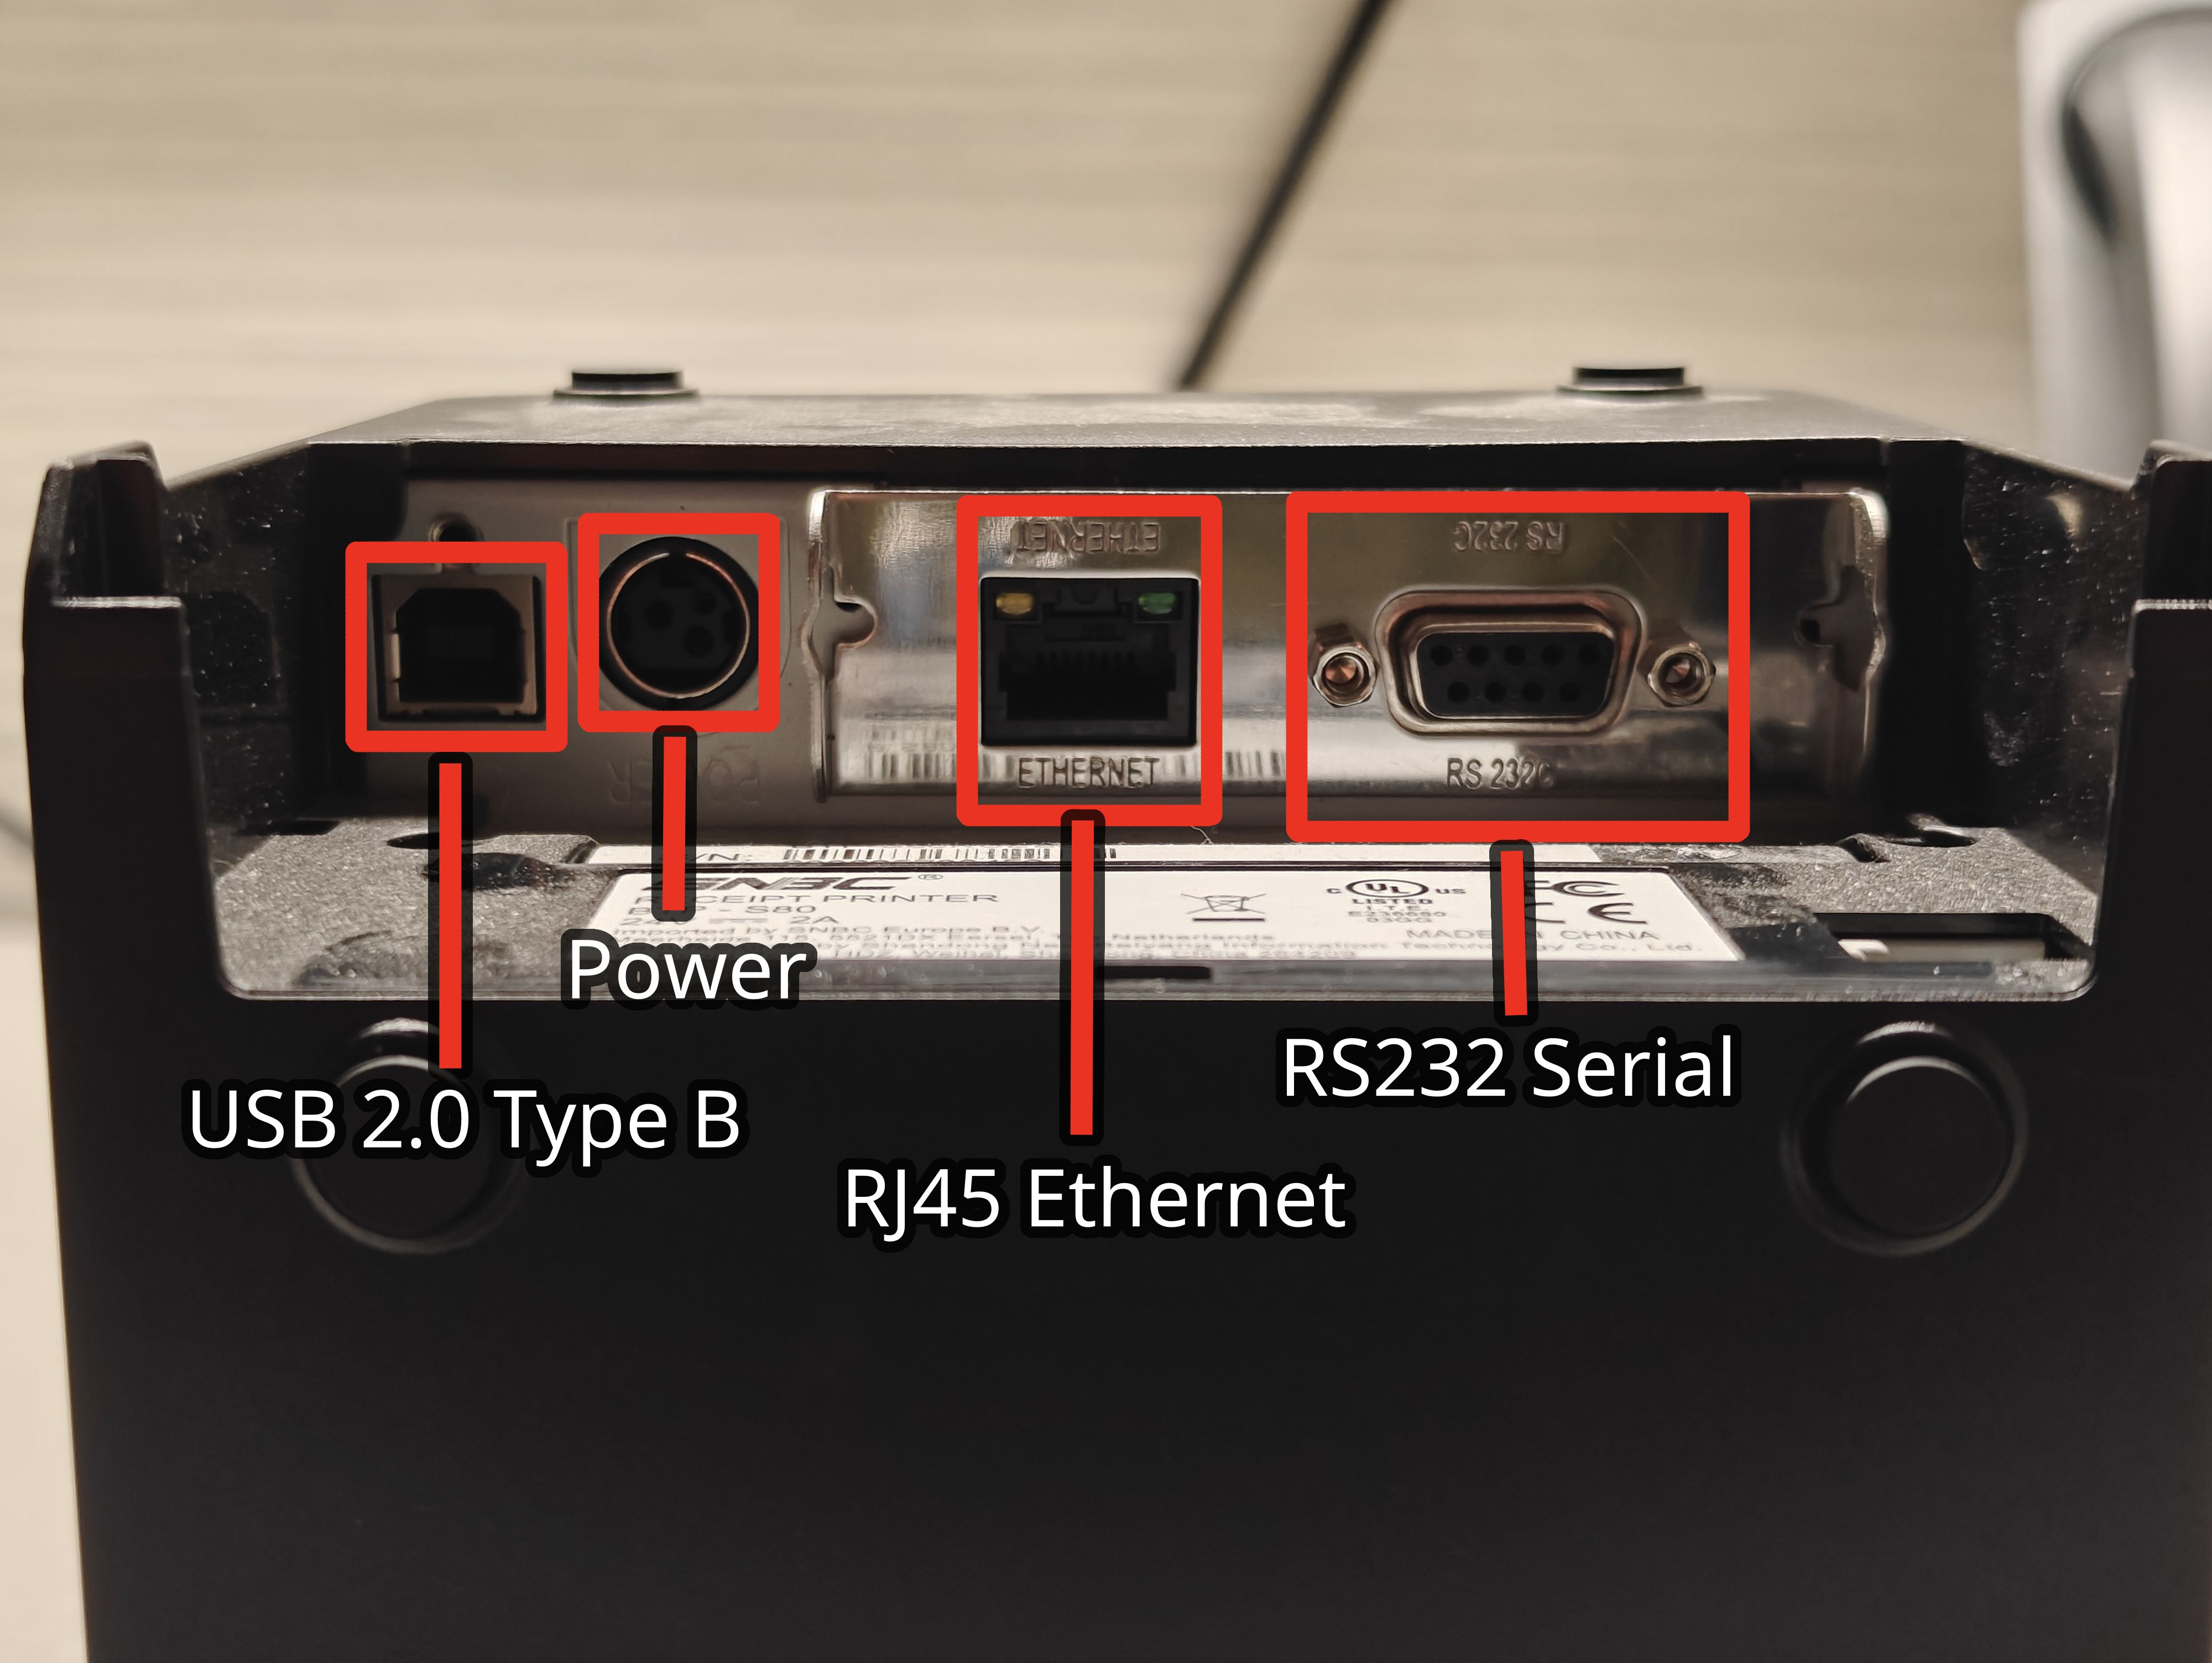
\includegraphics[width=88mm,scale=0.5]
    {Figures/Teardown/IMG20231204170442_annotated.jpg}}
    \caption{SNBC BTP-S80 labeled I/O}
    \label{fig:snbc_btp_s80_io}
\end{figure}

Removing each of the screws allows us to remove the chassis from the outer shell. Here we can see the motherboard (leftmost) and the expansion cards (topside, right of the motherboard). The expansion cards are divided into two parts, as shown in Figure \ref{fig:snbc_btp_s80_expansion}.

\begin{figure}[ht]
    \centering
    {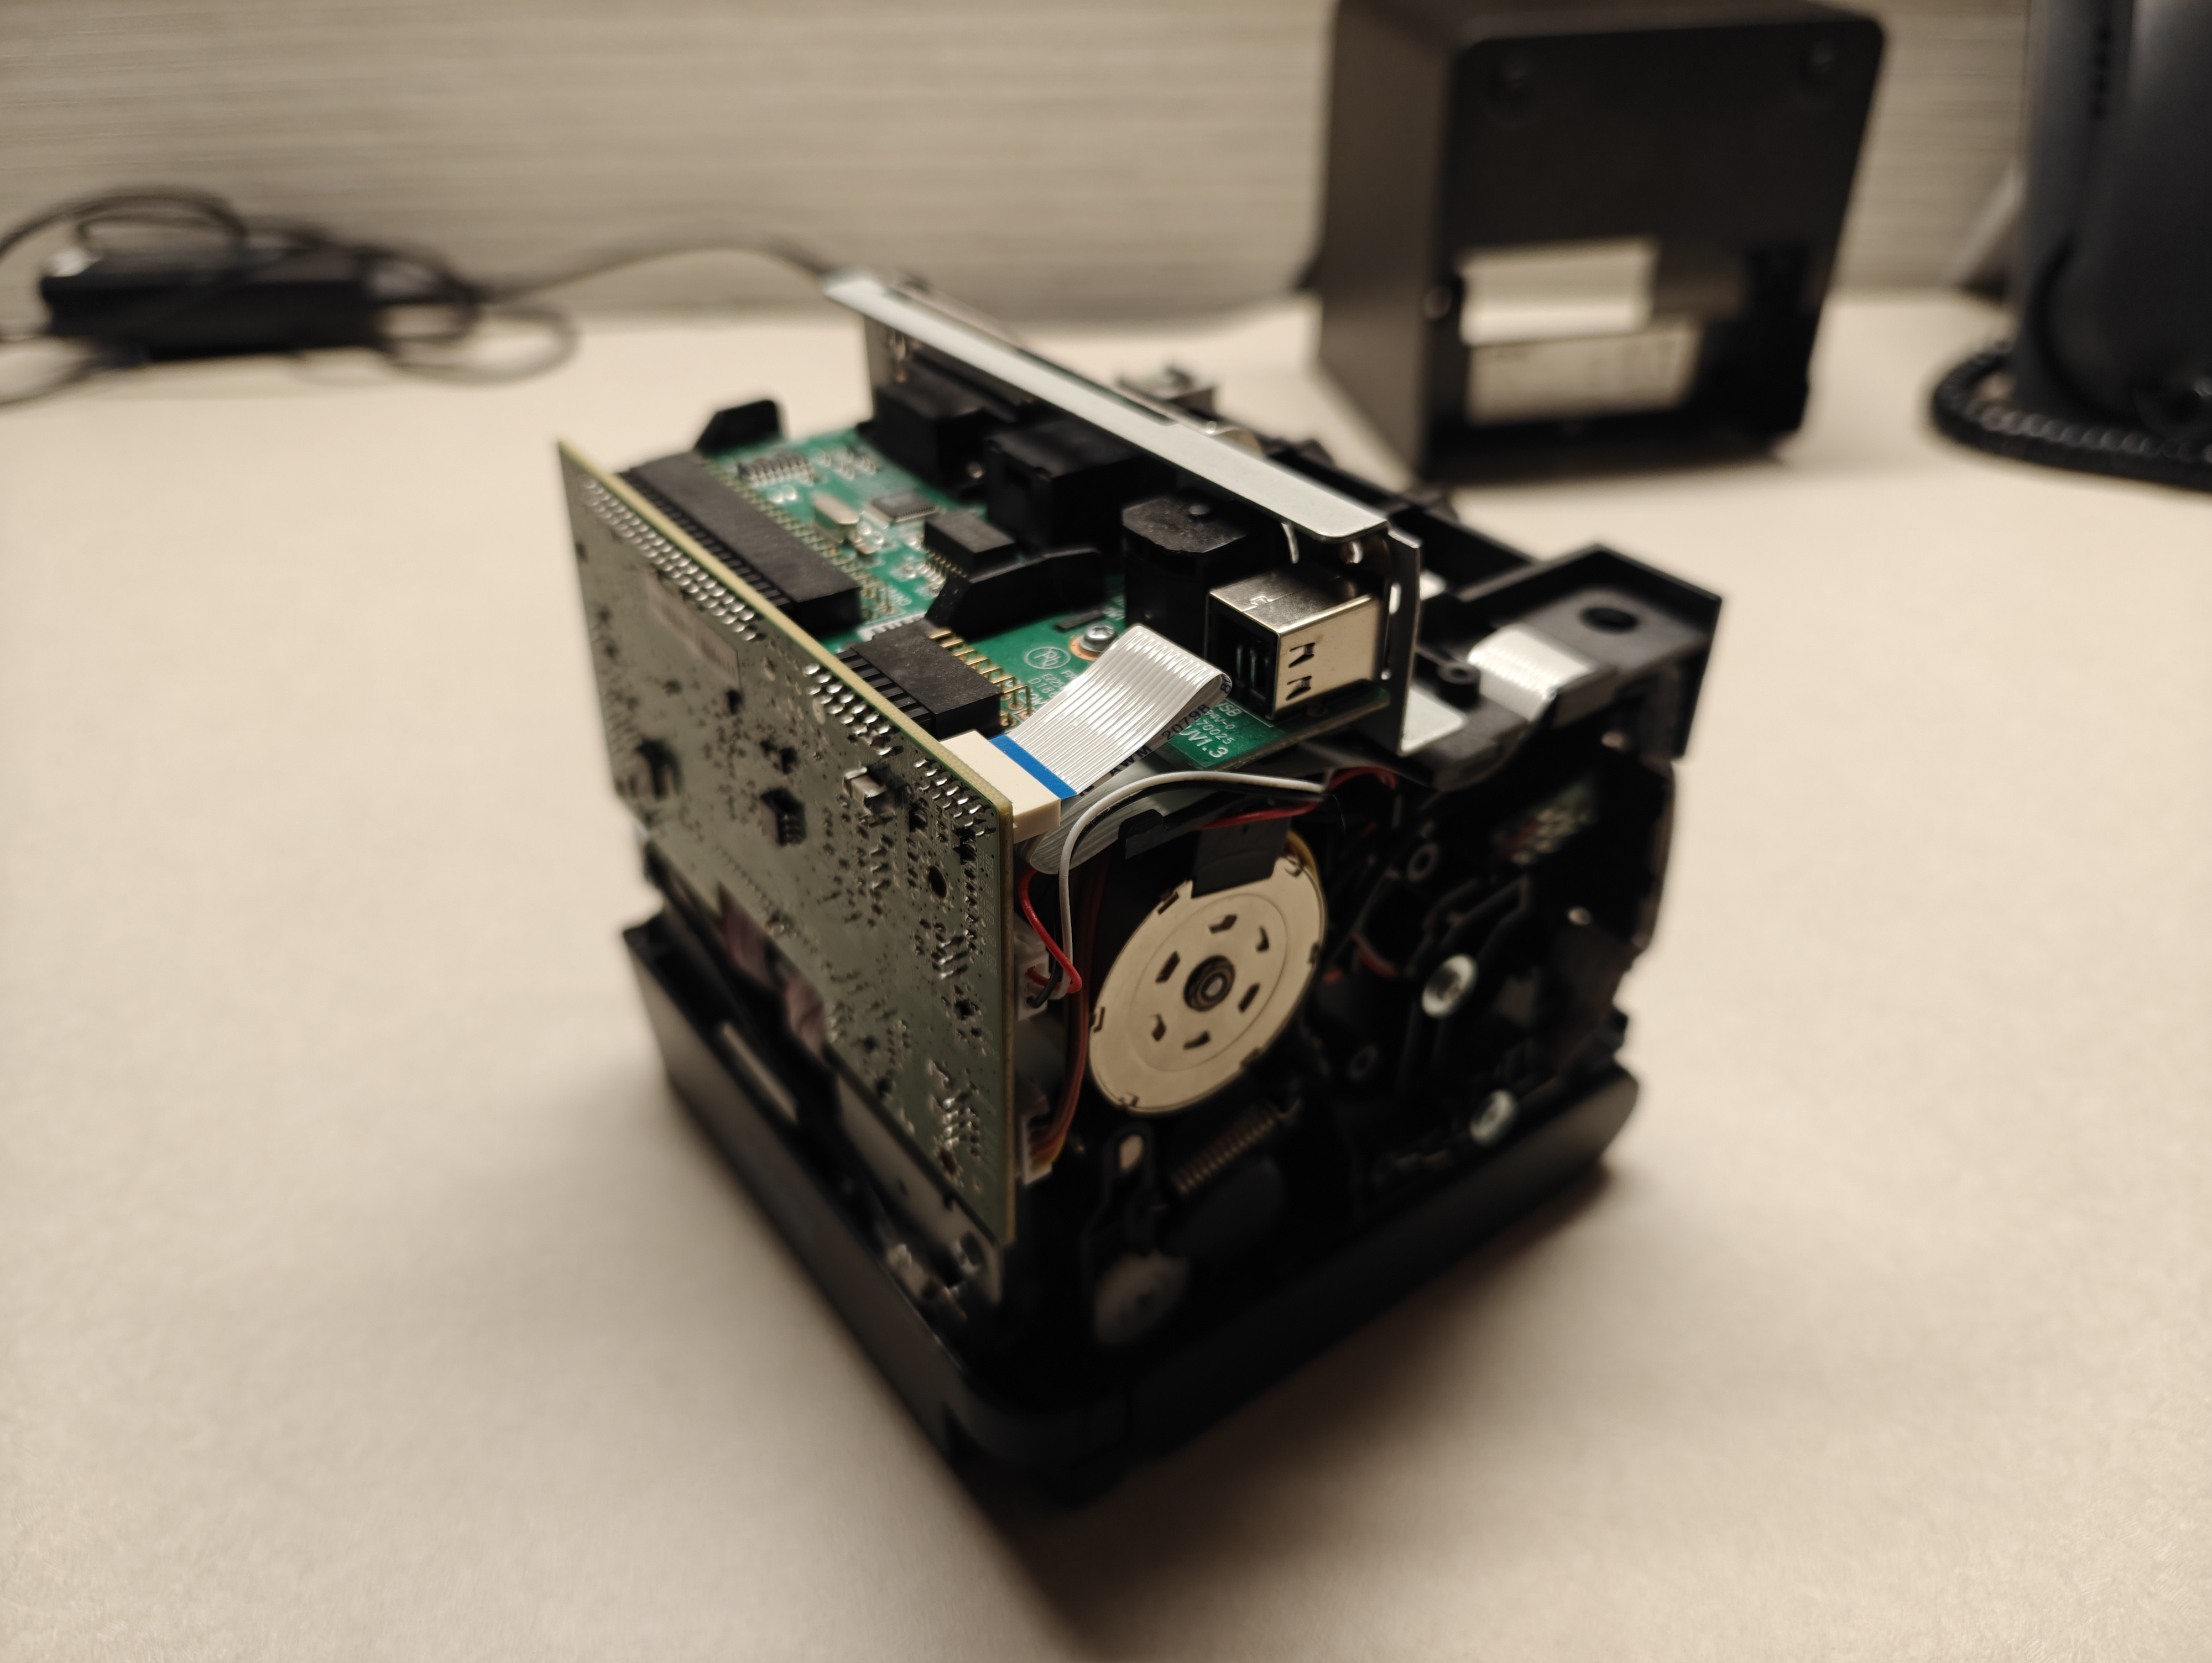
\includegraphics[width=88mm,scale=0.5]
    {Figures/Teardown/IMG20231204170938.jpg}}
    \caption{SNBC BTP-S80 inner chassis}
    \label{fig:snbc_btp_s80_chassis}
\end{figure}

The left expansion card allows the user of the device to swap networking stacks. In this configuration it features the RJ45 Ethernet and RS232 serial connector. The right expansion card provides USB connectivity and power via the barrel plug connector. 

\begin{figure}[ht]
    \centering
    {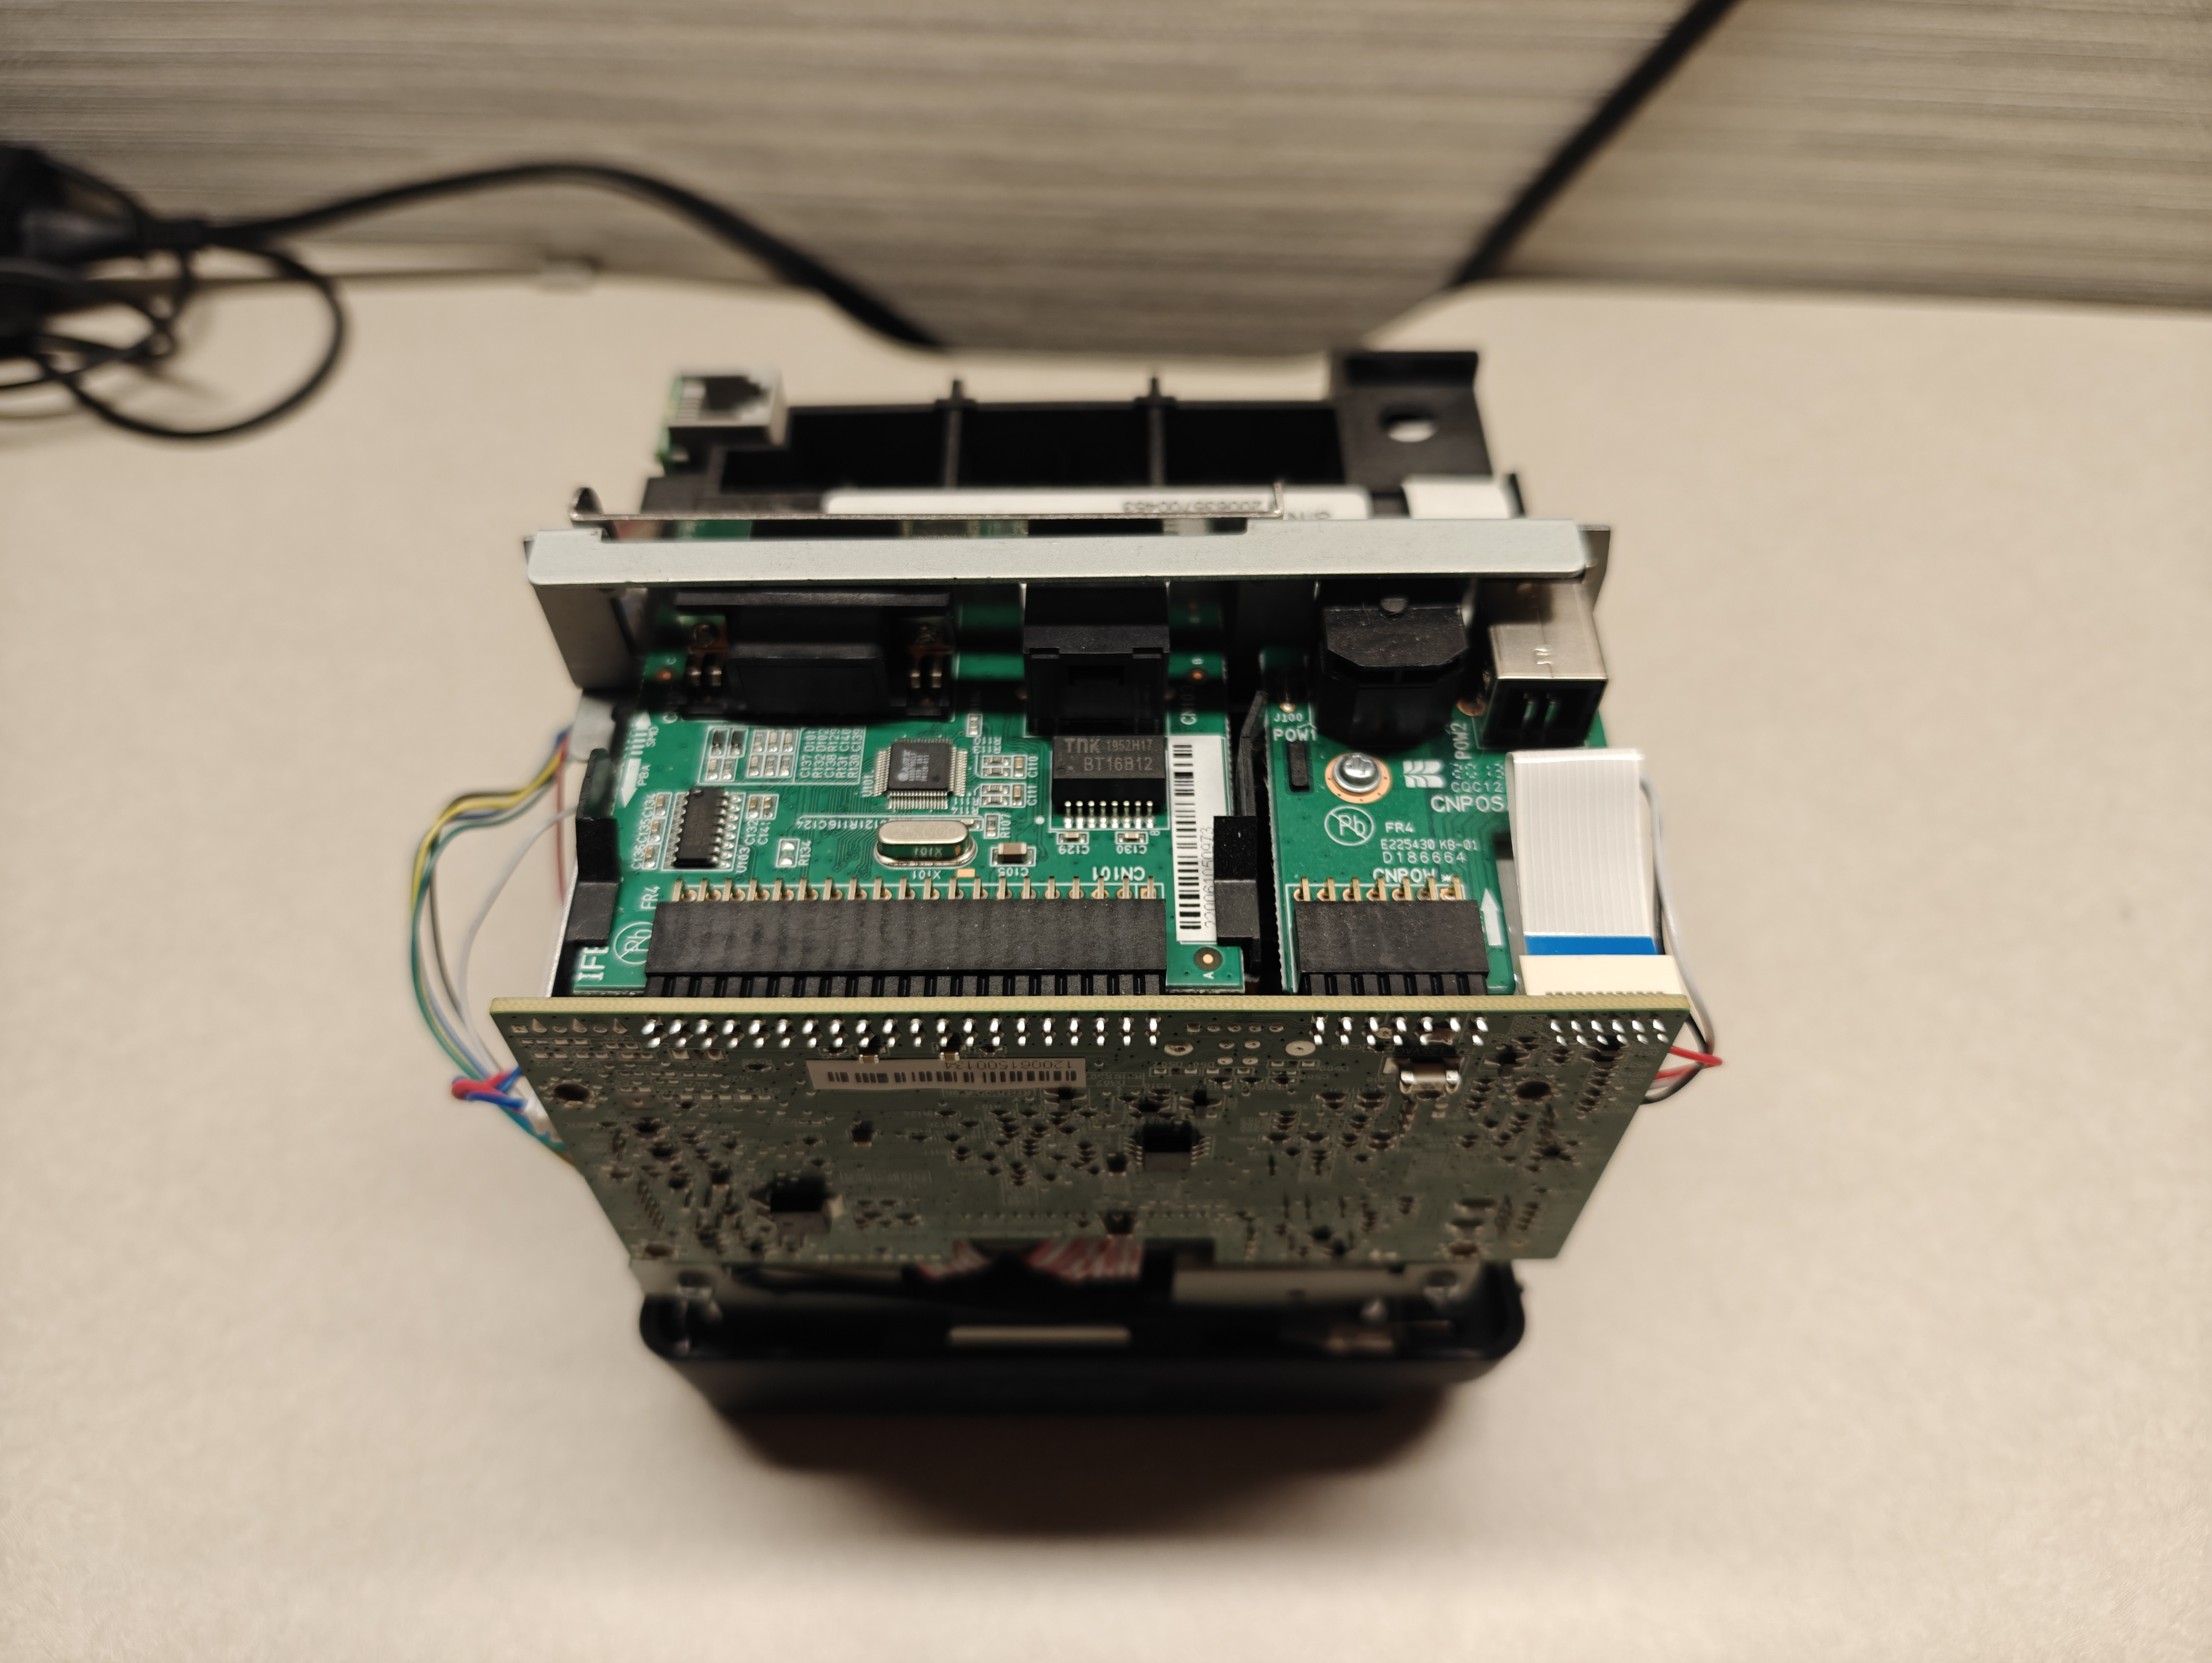
\includegraphics[width=88mm,scale=0.5]
    {Figures/Teardown/IMG20231204171002.jpg}}
    \caption{SNBC BTP-S80 expansion cards}
    \label{fig:snbc_btp_s80_expansion}
\end{figure}

The disassembly is completed after carefully disconnecting each cable, taking note of their respective connectors, and preparing the boards for component identification. There are plenty of components within the device, however, our concern is only the motherboard and two expansion cards. We are only interested in researching the components used for processing and storing data.


\subsection{Identified Components} \label{identifiedcomponents}


% \begin{itemize}
%     \item Walkthrough of documented teardown of the serial printer
% \end{itemize}

Component identification and analysis is divided into two parts. The first being analysis of the motherboard, and the second being the serial expansion card. Analysis of the power delivery and USB type-b expansion card is not necessary since it features no controllers nor any flash to analyze. In some cases, these might still be used for fuzzing and debugging because labeled connectors are provided, however, this can be ignored with most single wire debugging tools (e.g., Jtagulator or Bus Pirate).

\begin{figure}[ht]
    \centering
    {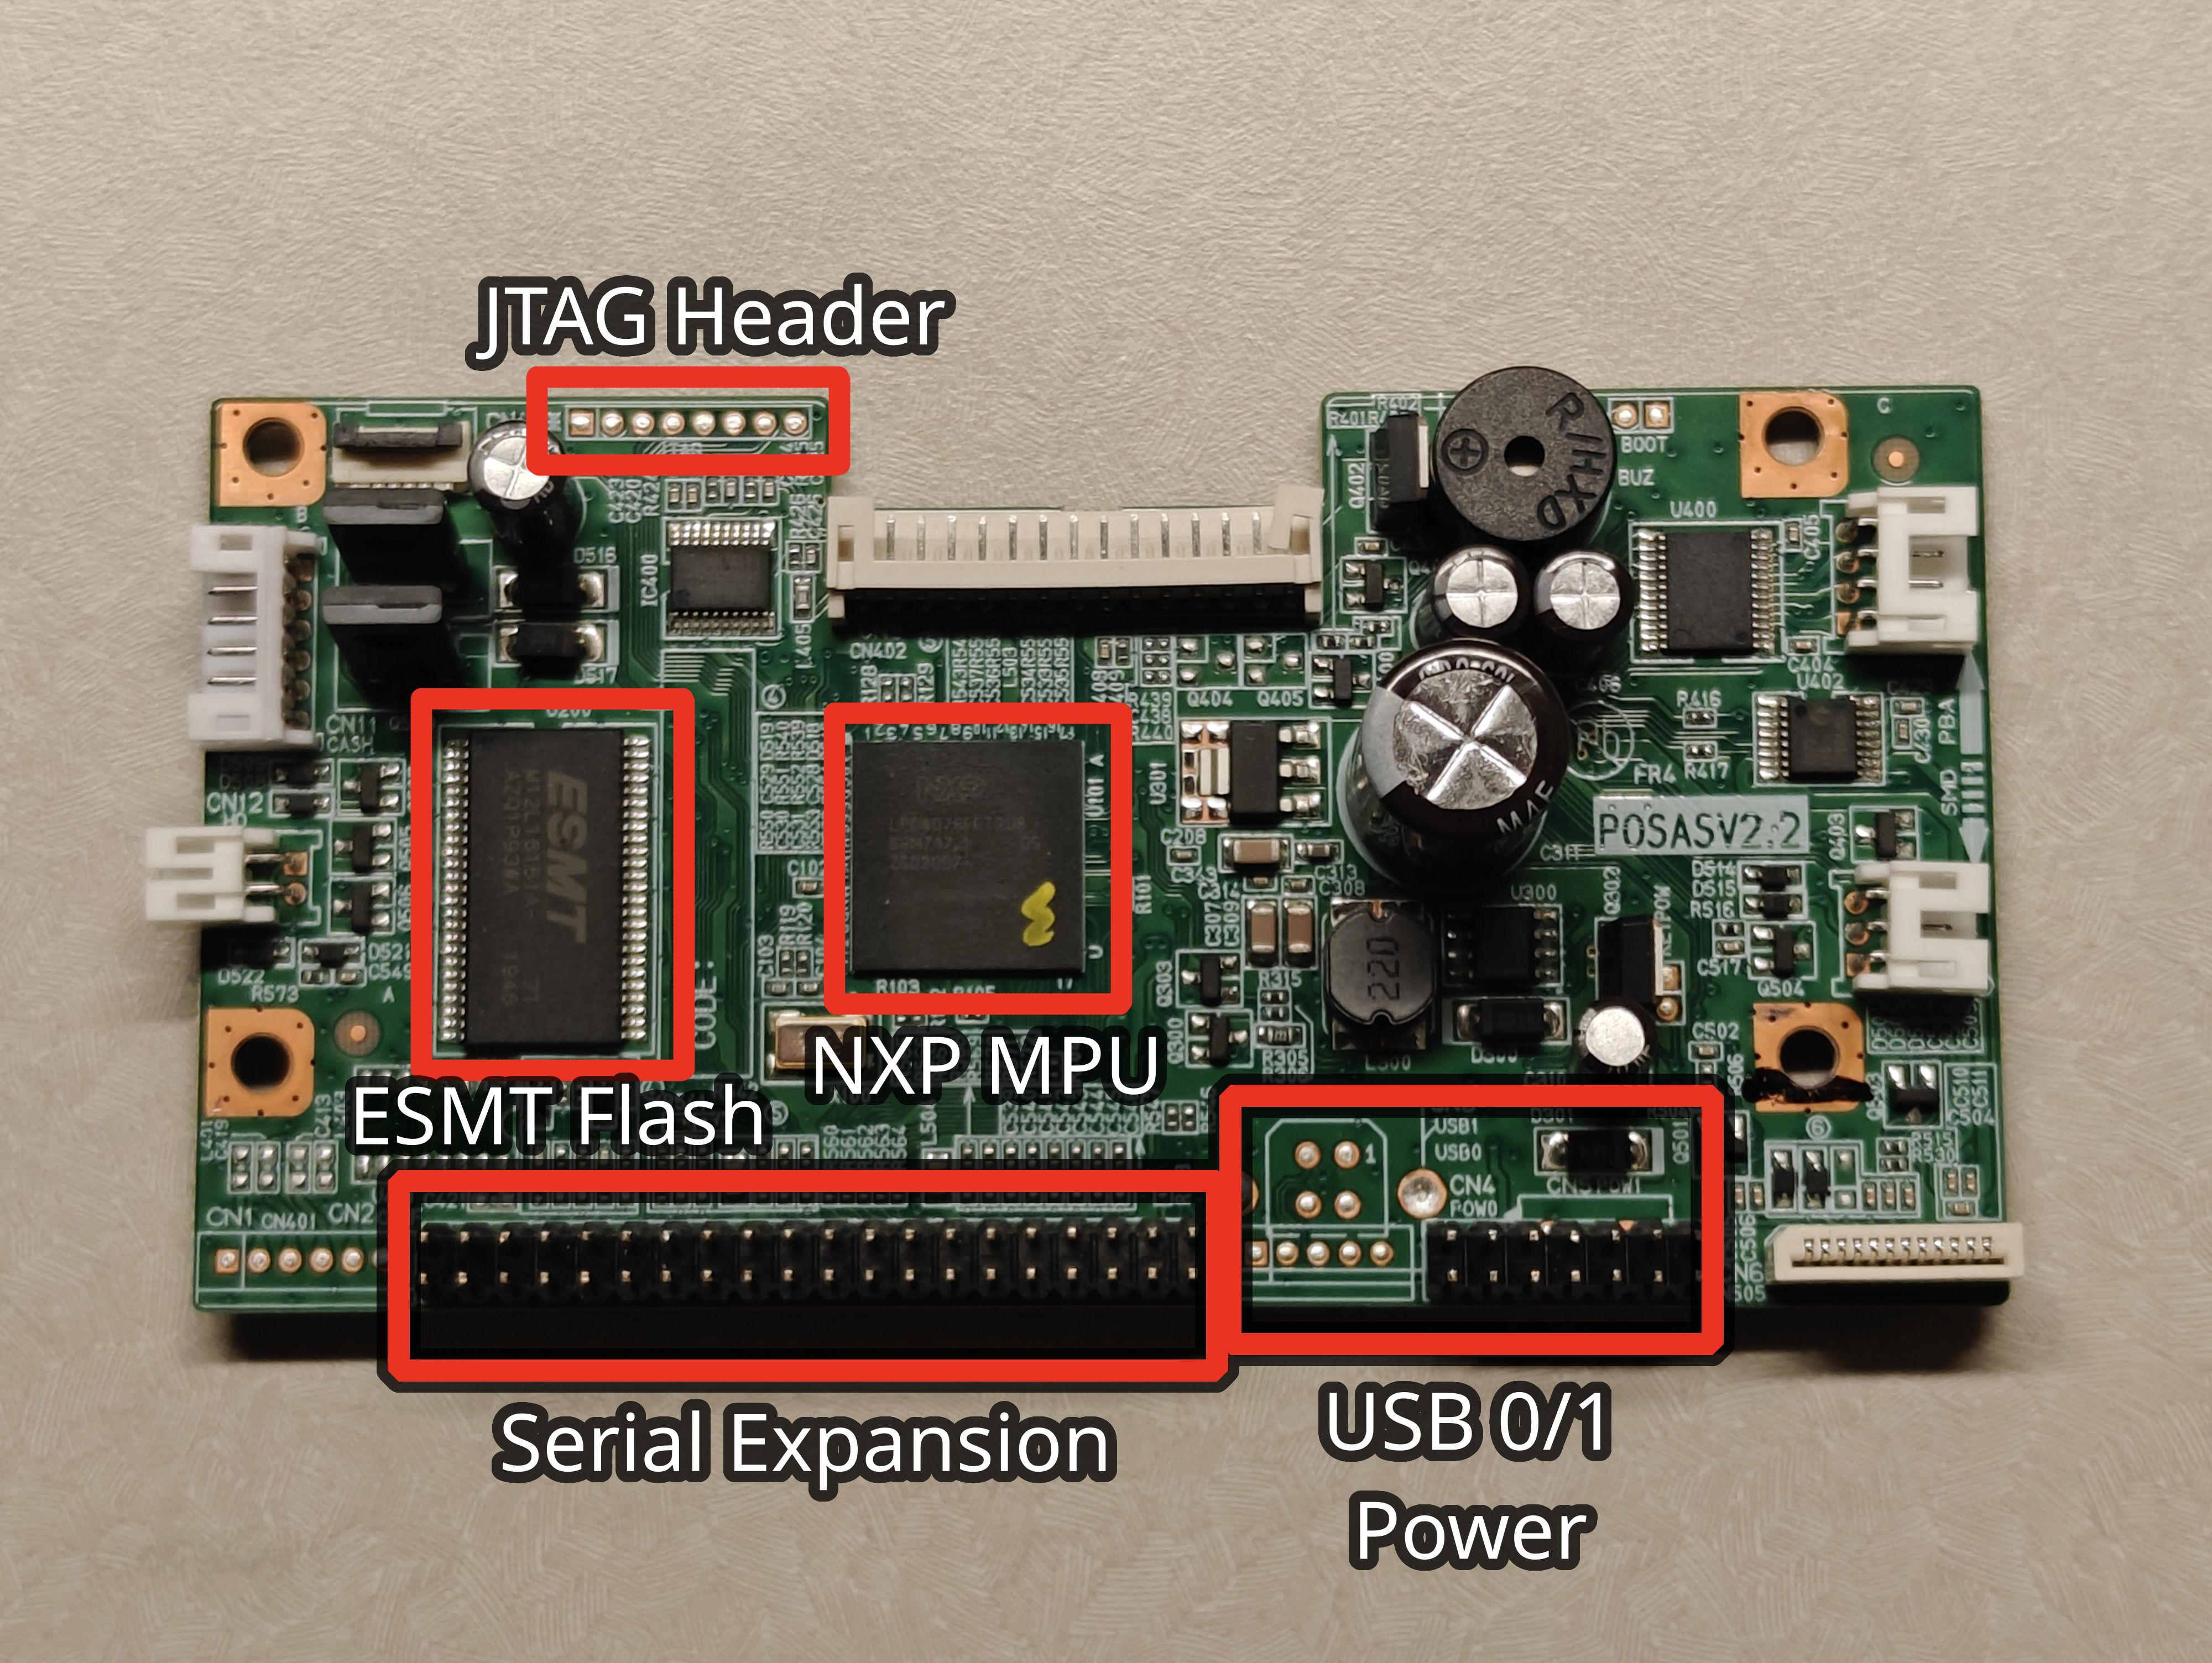
\includegraphics[width=88mm,scale=0.5]
    {Figures/Teardown/IMG20231204171516_annotated.jpg}}
    \caption{Motherboard components}
    \label{fig:snbc_btp_s80_motherboard}
\end{figure}

The list of motherboard components, as shown in Figure \ref{fig:snbc_btp_s80_motherboard}:
\begin{itemize}
    \item NXP MPU, 
    \item ESMT flash, 
\end{itemize}

\begin{figure}[ht]
    \centering
    {\includegraphics[width=88mm,scale=0.5]
    {Figures/Teardown/IMG20231204171204_annotated.jpg}}
    \caption{Expansion card components}
    \label{fig:snbc_btp_s80_expansion_components}
\end{figure}

The list of expansion components, as shown in Figure \ref{fig:snbc_btp_s80_expansion_components}:
\begin{itemize}
    \item SIPEX RS-232 Transceiver, 
    \item ASIX Ethernet Controller, 
\end{itemize}

Some words...

\subsection{Technical Resources} \label{technicalresources}

% List and describe datasheets and  source - AllDataSheets.com

\textbf{Outline}
$\downarrow$

\begin{itemize}
    \item List datasheets and where they were sourced
    \item Explanation of which sites/resources and why
\end{itemize}

pharetra sit amet aliquam id diam maecenas ultricies mi eget mauris pharetra et ultrices neque ornare aenean euismod elementum nisi quis eleifend quam adipiscing vitae proin sagittis nisl rhoncus mattis rhoncus urna neque viverra justo nec ultrices dui sapien eget mi proin sed libero enim sed faucibus turpis in eu mi bibendum neque egestas congue quisque egestas diam in arcu cursus euismod quis viverra nibh cras pulvinar mattis nunc sed blandit libero volutpat sed cras ornare arcu dui vivamus arcu felis bibendum ut tristique et egestas quis ipsum suspendisse ultrices gravida dictum fusce ut placerat orci nulla pellentesque dignissim enim.

\subsection{Firmware Analysis} \label{firmwareanalysis}

\textbf{Outline}
$\downarrow$

\begin{itemize}
    \item List bootloader information
    \item Details about recovered memory regions (e.g., addr ranges, size, perms)
    \item Known libraries
\end{itemize}

pharetra sit amet aliquam id diam maecenas ultricies mi eget mauris pharetra et ultrices neque ornare aenean euismod elementum nisi quis eleifend quam adipiscing vitae proin sagittis nisl rhoncus mattis rhoncus urna neque viverra justo nec ultrices dui sapien eget mi proin sed libero enim sed faucibus turpis in eu mi bibendum neque egestas congue quisque egestas diam in arcu cursus euismod quis viverra nibh cras pulvinar mattis nunc sed blandit libero volutpat sed cras ornare arcu dui vivamus arcu felis bibendum ut tristique et egestas quis ipsum suspendisse ultrices gravida dictum fusce ut placerat orci nulla pellentesque dignissim enim.

\subsection{Security Protections} \label{securityprotections}

\textbf{Outline}
$\downarrow$

\begin{itemize}
    \item Summary of physical protections (e.g., too much information silkscreened on PCB)
    \item List hardware protections (e.g., did manufacturer block debug access, are memory regions locked)
    \item Discuss software protections (e.g., access to bootloader, identifiable CVEs/CWEs, attributable libraries/functions)
\end{itemize}

pharetra sit amet aliquam id diam maecenas ultricies mi eget mauris pharetra et ultrices neque ornare aenean euismod elementum nisi quis eleifend quam adipiscing vitae proin sagittis nisl rhoncus mattis rhoncus urna neque viverra justo nec ultrices dui sapien eget mi proin sed libero enim sed faucibus turpis in eu mi bibendum neque egestas congue quisque egestas diam in arcu cursus euismod quis viverra nibh cras pulvinar mattis nunc sed blandit libero volutpat sed cras ornare arcu dui vivamus arcu felis bibendum ut tristique et egestas quis ipsum suspendisse ultrices gravida dictum fusce ut placerat orci nulla pellentesque dignissim enim.
